\documentclass[twocolumn]{article}
\usepackage{fullpage}
\usepackage{epsfig}
\usepackage{url}
\title{BoomFS: A Declarative Approach To Building\\Distributed Filesystems}
\author{Peter Alvaro, Neil Conway}
\date{December 19, 2008}
\begin{document}
\maketitle
\begin{abstract}
  While architectures for distributed computing are rapidly changing,
  techniques for building distributed systems have remained
  stagnant. As distributed computation becomes the common case,
  traditional techniques for building such systems will become
  untenable, because they force programmers to deal with the mundane
  details of constructing reliable distributed systems rather than
  concentrating on the desired computation. This yields programs that
  are difficult to construct, understand, modify, and adapt to new
  environments. We propose BOOM, an ongoing project to develop concise
  declarative specifications for a broad class of scalable distributed
  systems. In this paper, we describe the first application in the
  BOOM stack: BoomFS, a distributed filesystem that is implemented
  using a combination of Java and declarative logic. We show that
  BoomFS is easy to understand and modify, and achieves competitive
  performance in a preliminary performance study.
\end{abstract}
\section{Introduction}
\label{introduction}
With the widespread adoption of cloud computing, mobile clients, and
manycore processors, computing architectures are undergoing a period
of disruptive change. In the near future, nearly every non-trivial
software system will be physically dispersed: distributed programming
will be the common case.

Traditional techniques for building distributed systems are ill-suited
to this new environment. Despite considerable research, developing
fault-tolerant distributed systems remains enormously difficult and
expensive, and is typically only attempted by experienced programmers
with extensive training in the field. As more journeyman developers
begin to encounter the challenges of distributed computing as a matter
of course, this situation will become increasingly untenable. Better
techniques for constructing distributed systems are urgently needed.

Inspired by prior work on declarative networking~\cite{dn-sigmod,
  network-data-indep}, we propose a new architectural style for
distributed programs in which policy and protocol are specified in a
declarative logic language, while the operational mechanisms of the
program are written in a traditional imperative language. We are
engaged in the Berkeley Orders of Magnitude (BOOM) project, which aims
to use this style to build cloud computing infrastructure components
that operate at orders of magnitude greater scale but are specified in
orders of magnitude less code than traditional approaches. In Section
\ref{boom-vision}, we discuss the problems with traditional approaches
to building distributed systems in more detail, and outline the BOOM
vision in contrast.

The first system we have built using this architectural style is
BoomFS, a distributed filesystem similar to the Google File
System~\cite{gfs}. Our goal in building this system was not novelty of
design: although BoomFS supports multiple master nodes, its
architecture is otherwise very similar to GFS. Instead, our aim was to
show that a GFS-like filesystem can be easily and concisely
implemented in the BOOM style. The resulting system should achieve
competitive performance, and be easy to understand and adapt to new
environments and policies. In Section \ref{system-arch}, we describe
the basic architecture of BoomFS. In Section \ref{system-realize}, we
detail how this architecture was realized using a mixture of
declarative logic and Java. In Section \ref{perf-eval}, we report on a
preliminary performance study comparing BoomFS and the Hadoop File
System (HDFS), an open source implementation of
GFS~\cite{hdfs-arch}. We discuss plans for future work in Section
\ref{future-work}, describe related research in Section
\ref{related-work}, and conclude in Section \ref{conclusion}.

\section{The BOOM Vision}
\label{boom-vision}
The fundamental problem with traditional techniques for building
distributed systems is that they provide the wrong abstractions to the
programmer. Distributed systems are typically implemented with tools
developed for single-machine programs and only superficially adapted
to the challenges of a distributed setting. Programmers are forced to
deal with the tedious details of communication, synchronization, and
consensus. As a result, the essence of the distributed computation is
obscured by a forest of boilerplate details. Evidence for this can be
seen in the fact that distributed algorithms such as Paxos can be
stated in a page of pseudocode, but require many thousands of lines of
code to implement using standard tools~\cite{paxos-made-live}.

Traditional tools operate at a low level of abstraction because they
force programmers to intermingle the specification of \emph{what} a
distributed program should do with \emph{how} it should be
achieved. That is, mechanism and policy are specified together, and
implemented in the same language. This approach has two primary
problems: it yields fragile programs that cannot easily adapt to
change, and it results in programs that are difficult to understand.

For example, consider a client that wants to compute a function over
data stored in a compute cloud. Should the function's code be sent to
the server, should the data be sent to the client, or should both code
and data be sent to an intermediary? These alternatives can be viewed
as ``query plans'' that accomplish the same objective, but have
different performance characteristics. The optimal plan depends on
factors including the relative costs of network bandwidth, server-side
computation and client-side computation, how much data is required,
how expensive the function is, and the frequency with which the
function is invoked or the input data is modified. All of these
parameters are likely to fluctuate, both within a single environment
over time,\footnote{Internal heterogeneity and performance variability
  in virtualized environments such as Amazon's Elastic Compute Cloud
  has been well-documented in recent work~\cite{late-sched}.} and when
the distributed program is deployed to a new environment. Traditional
approaches to constructing distributed systems require hardcoding
assumptions about these parameters. This yields fragile programs that
are expensive to modify and difficult to adapt to new environments.

In addition to being inflexible, the failure to separate mechanism from
policy it harder to understand and reason about these programs. The
policies and protocols of a distributed program are typically its most
interesting parts, and often the hardest to get right. In contrast,
the mechanisms that achieve those policies are often straightforward
but verbose. By implementing policy together with mechanism, the
mundane details of the latter obscure the essential nature of the
former, harming comprehensibility. Furthermore, a language that is
appropriate for implementing mechanism is unlikely to be ideal for
specifying policy, and vice versa. There are many examples of
algorithms that can be concisely expressed in an appropriate
declarative language, but are much harder to write in an imperative
language (e.g.\ \cite{chord-overlog}).

Inspired by the data independence provided by the relational model, we
aim to provide \emph{network scale independence} for distributed
systems by separating the programmer's intent from its concrete
realization. In BOOM, a distributed system is composed of two types of
components:
\begin{enumerate}
\item
  \emph{imperative} components implement the basic units of
  functionality of a distributed system. Imperative components are
  typically used to perform tasks like I/O and numerical
  computation. These tasks are usually best stated in an imperative
  language like Java or C++, particularly because these components
  often involve interaction with the operating system or native
  libraries.

\item
  \emph{declarative} components specify the bulk of the logic of the
  distributed system. These components are written as a collection of
  logical rules that describe the coordination and composition of the
  imperative components. Essentially, the declarative components are
  responsible for deciding ``what'' a member of the distributed system
  should do; the imperative components are responsible for realizing
  those actions. A declarative component is essentially a join between
  a stream of events and a database. Evaluating this query over an
  event stream results in producing more events (either at the local
  node or a remote node), inserting new database tuples, or invoking
  imperative components.

  Declarative components are implemented in a network-aware
  declarative logic language, such as Overlog~\cite{dn-sigmod}. This
  requires the state of the distributed program to be represented as
  relations that are partioned over the nodes of the system.
\end{enumerate}

In BoomFS, imperative components are used to efficiently transfer data
between hosts. The vast majority of the filesystem's complexity
resides in the declarative components, which decide when and where
data should be transferred. We describe the realization of BoomFS as a
set of imperative and declarative components in Section
\ref{system-realize}.

\subsection{Declarative Specification of\\Distributed Filesystems}
In many systems, there is a structural separation between control and
data paths. This can be motivated either by principle (the separation
of mechanism and policy~\cite{hydra-policy-mech-sep}), or by practical
concerns: data and control paths typically differ in average message
size, and in requirements for consistency and latency. It is
undesirable for data path congestion to delay control messages.

We argue that in many distributed systems, the bulk of the
intellectual complexity resides in the control path; this is clearly
true of the GFS design. This is not to say that operational components
(zero-copy I/O, fast checksumming, careful use of caches at various
levels) are not critical to system performance, but merely that the
bulk of the design and implementation deal with enforcing and
maintaining the various invariants that make the system behave
correctly, including replica placement decisions, failure handling,
load balancing and consensus among agents in shared computations.

Combining these observations, we see that the GFS style of distributed
filesystem is a perfect testing ground for the BOOM approach to
implementing distributed systems.

\section{System Architecture}
\label{system-arch}
We now turn to the architecture, implementation, and performance
characteristics of BoomFS. The architecture of the system is directly
inspired by the Google File System. The design goals and system
architecture of GFS are well-documented elsewhere~\cite{gfs,
  hdfs-arch}, so we include only a brief discussion of them here.

Like GFS, BoomFS does not attempt to be a general-purpose distributed
filesystem. Instead, it is designed to perform well for a particular
class of workloads, and to operate on a particular cluster
architecture. We focus on achieving good performance for large
sequential reads and writes. Files are assumed to be very large, and
are therefore divided into large \emph{chunks} that far exceed typical
filesystem block sizes (64MB). We focus on
delivering high sequential read and write throughput and efficient
network utilization, rather than achieving low latency or minimizing
total disk space requirements. Members of a BoomFS system are assumed
to be unreliable commodity machines, provisioned with relatively
modest resources.  Reliability is achieved by storing multiple copies
of each chunk; scalability is achieved by spreading filesystem
contents over a large cluster of machines (typically hundreds or
thousands).

\begin{figure}
\centering
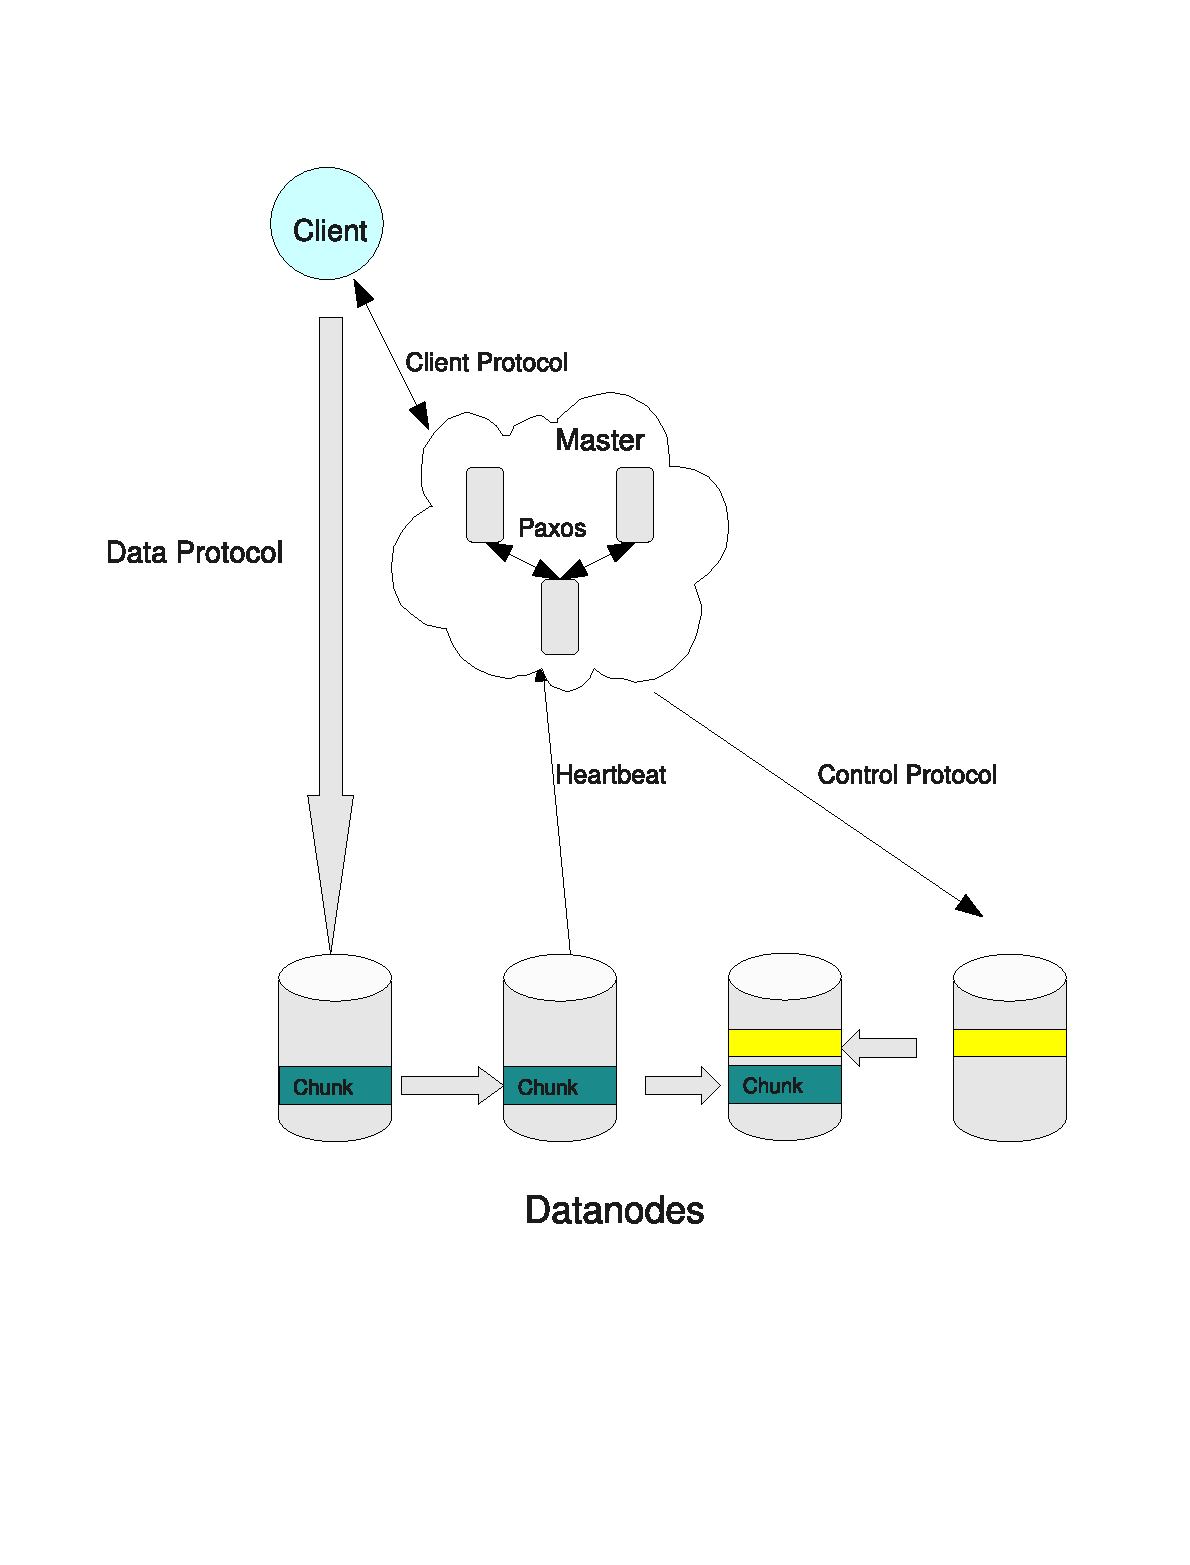
\epsfig{file=figures/arch.eps, width=1\columnwidth}
\caption{BoomFS architecture}
\label{fig:system-arch}
\end{figure}

\subsection{System Overview}
The major components of BoomFS are depicted in Figure
\ref{fig:system-arch}. There are three types of nodes in BoomFS:
\emph{master nodes}, \emph{data nodes}, and \emph{clients}. Master
nodes contain the canonical description of the structure of the
filesystem. The filesystem is described by a mapping from file names
to file identifiers, and from file identifiers to the sequence of
chunks that contain the file's content. To avoid a single point of
failure, our design allows for multiple master nodes, which are kept
in synchrony using a consensus protocol (currently
Paxos~\cite{paxos-made-simple}).

Data nodes are responsible for storing chunks. They have no knowledge
of the structure of the filesystem as a whole, or of the files to which  
the chunks they store belong.  Nor do they have any \emph{a priori} knowledge
of the identities of other data nodes in the system;  these are explicitly
specified in the data path protocol.  Each data node periodically sends a
\emph{heartbeat} to the master nodes. This notifies the masters that
the data node is still alive, and contains a list of the chunks
currently stored at the data node. The masters use this information to
update a mapping from chunk identifiers to the set of data nodes that
might be holding that chunk. Note that the canonical description of
the content of a data node resides at the data node itself, not at the
master nodes; the master's copy of this information is updated lazily.

Finally, client nodes represent application programs that wish to read
and write files. We expect that applications will interact with the
system through a client library that provides a convenient stream-like
abstraction for files stored in BoomFS. In the future, we plan to
implement the HDFS API, to allow BoomFS to easily replace HDFS in
existing Hadoop installations. % mention POSIX?

\subsection{Filesystem Operations}
\label{fs-ops}
To append to a file, a client node begins by contacting one of the
master nodes, and requesting that a new chunk be added to a particular
file.\footnote{In the current prototype, random writes are not
  supported, and each append operation creates a new chunk --- we
  expect that each append will be large enough to justify occupying an
  entire chunk. We plan to relax this constraint in the future.} The
master first generates a new chunk identifier. To ensure that the
state of the file system is consistent across all the masters, the
master uses a consensus protocol to ensure that all masters have
agreed to add the new chunk identifier at the same position in the
chunk list for the appropriate file. Once consensus has been reached,
the master replies to the client with the new chunk identifier, and a
list of data nodes that might be appropriate locations for the new
chunk.

The client is then responsible for pushing data for the chunk to a
sufficient number of data nodes. There are various policies a client
could use to do this. For example, the client could directly connect
to all the data nodes and send the chunk content itself, or it might
only send the data to a single data node, and instruct that node to
propagate the data onward. Once the content of a chunk has been
completely received by a data node and written to disk, this fact will
be reflected in the next heartbeat that the data node sends to the
masters. In turn, this will make the data node available for
subsequent operations on the chunk.

To read a file, a client once again begins by contacting one of the
master nodes to fetch the list of chunks that make up the target
file. For each chunk identifier in the list, the client consults the
master to determine the set of data nodes that have copies of that
chunk. The client then reads the chunk by connecting to one of the
data nodes directly.

To delete a file, a client contacts a master node. The master passes
the request through the consensus protocol. When consensus has been
reached, all the masters remove the file from their internal
metadata. There is no need to eagerly contact data nodes to remove the
chunks belonging to the deleted file: the next time the data node
sends a heartbeat to a master, the master replies with a list of the
chunks on the data node that is has no knowledge of. These orphaned
chunks can be garbage collected at the data node's leisure.

Other filesystem operations are straightforward. For example, clients
interact with master nodes to obtain directory listings, and create
and remove directories.\footnote{Our prototype implementation of
  BoomFS does not currently support directories, but we expect that
  this implementation shortcut will be easy to fix.}

\section{System Realization}
\label{system-realize}
The filesystem design described in Section \ref{system-arch} is
abstract, and might reasonably be implemented using a variety of
techniques. In this section, we describe how we realized the BoomFS
design using a combination of Java and Overlog. In the following
discussion, we assume that the reader has some familiarity with
Overlog~\cite{dn-sigmod}.

We validate this implementation strategy in two ways: by demonstrating
how this implementation allows for the easy modification of filesystem
policies in Section \ref{decl-approach}, and by conducting a performance
study in Section \ref{perf-eval}.

\subsection{Software Architecture}
% \begin{figure}
% \centering
% 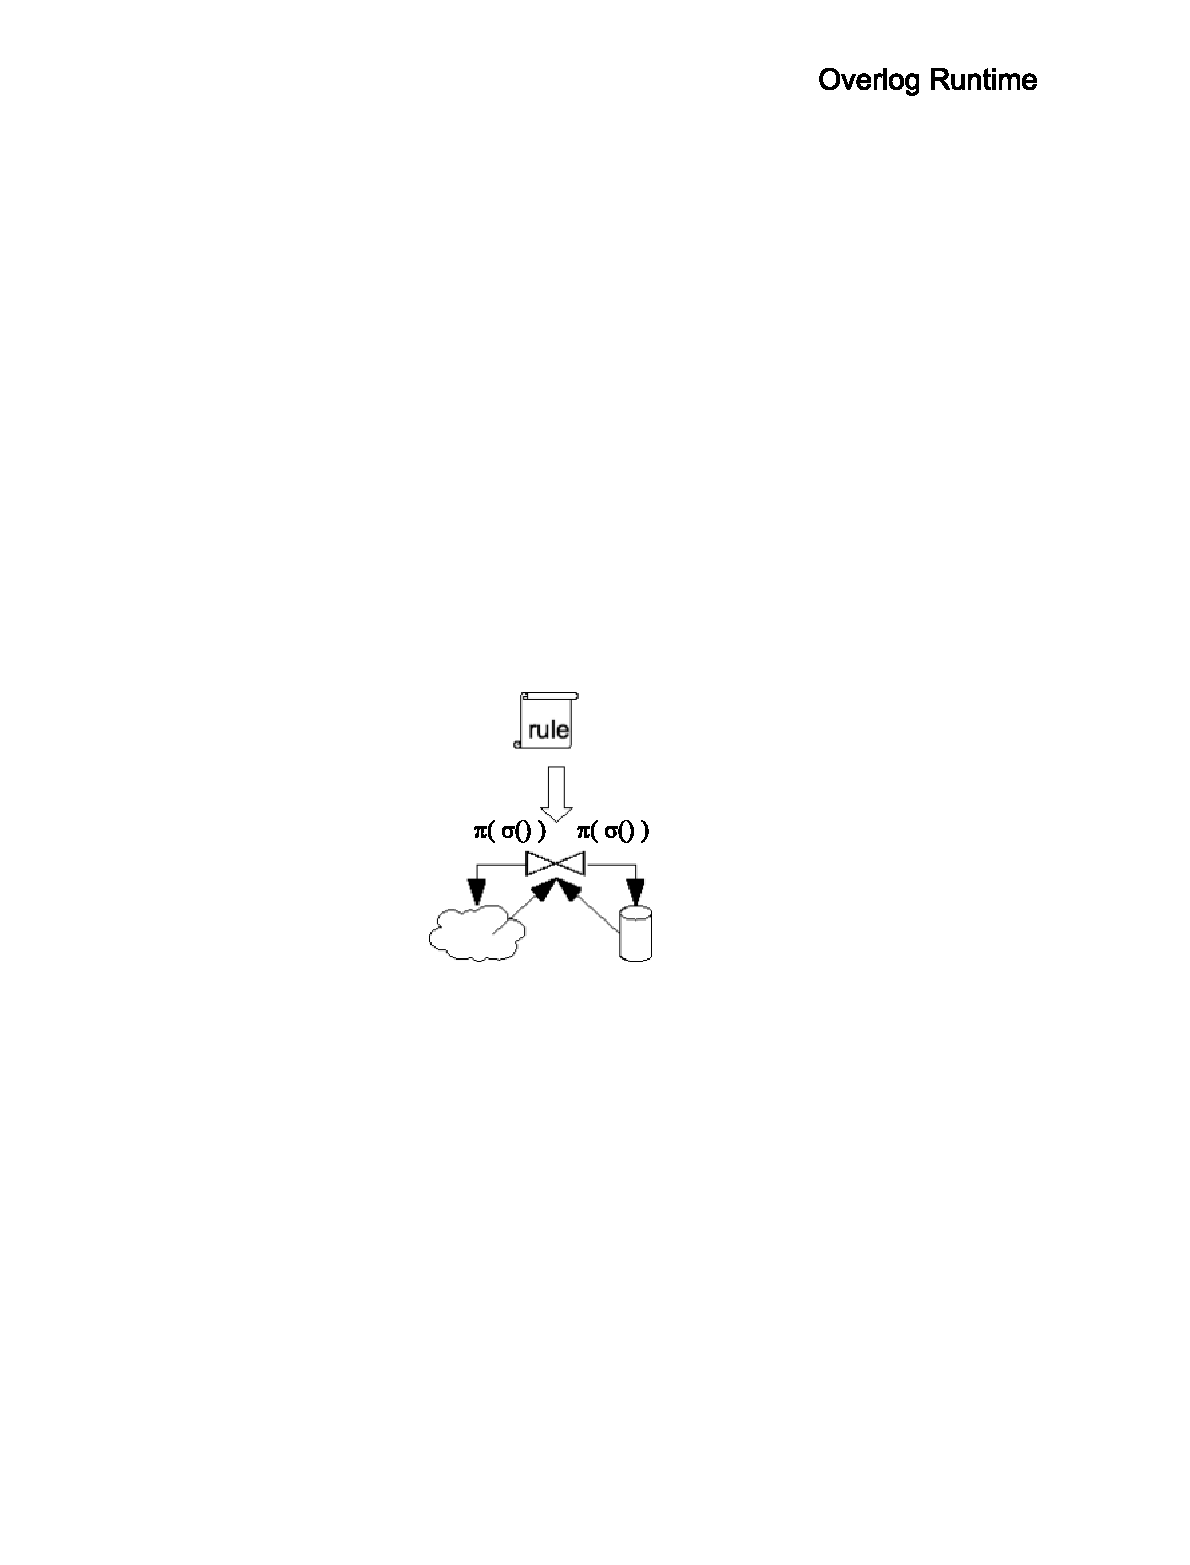
\epsfig{file=figures/dataflow.eps, width=1\columnwidth}
% \caption{The architecture of a program using JOL}
% \label{fig:jol-arch}
% \end{figure}

In BoomFS, masters, data nodes, and clients are all implemented using
a combination of Java and Overlog. We used JOL~\cite{jol}, a
Java-based Overlog implementation that allows an Overlog evaluator to
be embedded inside a Java program, and allows Overlog programs to
contain Java objects and invoke Java methods. Java programs can insert
and delete tuples from Overlog relations, and register ``queries''
that invoke a callback when a particular state is reached by the
Overlog instance.

Each node type in BoomFS is structured in a similar way. Upon startup,
the node runs Java code that bootstraps a JOL instance, and installs
the Overlog files for BoomFS.

This architecture is quite similar to the familiar structure of an
application that uses a DBMS: the database is responsible for managing
data, and the application uses queries to retrieve and modify the
state of the database. However, there are some crucial differences
between this architecture and the design of BoomFS. For example,
Overlog relations are partitioned over multiple nodes.  While one-time
queries are expressible in Overlog, continuous queries are the more
common case, represented syntactically as a recursive join and
semantically as a cyclic dataflow graph.

\subsection{State Representation}
Any filesystem contains two kinds of state: data and metadata. In
BoomFS, data is stored as a collection of chunks distributed over the
data nodes. Each data node stores chunks as normal files on its
local filesystem.

All the metadata in BoomFS is represented as relations; some of these
relations are partitioned over multiple nodes.

\subsection{Control Path}
\label{control-path}
In GFS, the control path comprises three separate protocols: the
client protocol spoken between clients and masters to modify
filesystem metadata, the control protocol between master and data node
used for replica migration or deletion instructions, and the
heartbeats regularly sent from data nodes to the masters.  The
replication mechanism, which in GFS involves a log flush to multiple
slave masters, can be considered a fourth protocol.

In our design, instead of using separate state machines to implement
the various communication protocols, all control path messaging is
specified declaratively.  Logical inference rules, like database
views, perform select-project-join over locally materialized
relations, and the newly projected tuples are sent over the network if
their location specifier indicates that they belong in a different
partition, and hence a different node in the system.  At the
destination, an incoming tuple's schema describes its content and
determines which rules, if any, should be reevaluated with reference
to the new data.

For read-only operations like many client protocol interactions, a
single declarative rule on the client (to transfer the injected
request tuple to the master) and a pair of rules on the master (one to
return the results to the client, and an error handler) suffice to express the messaging logic.
Requests that modify filesystem metadata follow the same structure,
but trigger a more complicated chain of inferences on the master.  In
particular, the master must achieve consensus among master replicas,
attempt the modification, and indicate success to the client only if
these steps succeed.  Heartbeats from data nodes to the master are
structured similarly to client requests, but are triggered by a
periodic timer rather than by human interaction.  Finally, control
protocol messages from master to data node are fired when conditions
specified by certain aggregate queries indicate that system invariants
are unmet, as when the number of replicas drops below the specified
replication factor.

Let us take a concrete example beginning with a client request to
append a stream of data to a file.  The Java shell code running at the
client injects a tuple into a local table, triggering a send rule that
causes the tuple, which contains the client's address, the file
identifier, and a opcode indicating that this is a request for a new
chunk identifier, to the master.  This initiates a chain of inferences
that generate a new id, achieve consensus on the assignment of this id
to the given file's list of chunks, and select a set of possible
candidate data nodes that may store the new chunk.  The resulting
chunk identifier and candidate data node list are then embedded in a
tuple and returned to the client.  The client applies its local
policy, which may be a simple distance function, to sort the set of
candidate data nodes and select a next hop.  From here, the data path
is invoked for the remainder of the operation.

\subsection{Data Path}
The data protocol is a straightforward mechanism for transferring the
content of a chunk between two hosts. The server side of the protocol
is implemented as a simple imperative component that runs on each data
node. It listens on a dedicated TCP port and handles each client
connection using a separate thread. Data transfer is done using the
\texttt{FileChannel.transferTo()} mechanism provided by Java NIO,
which allows an underlying zero copy API to perform the bulk data
transfer (such as \texttt{sendfile(2)} on Linux). The data protocol
consists of two simple operations: writing a chunk from the client to
the server, and reading a chunk from the server to the client. The
protocol client is either a client node or another data node.

While the data protocol is unicast, a client node typically wants to
write a new chunk to multiple data nodes. As noted in Section
\ref{fs-ops}, there are several ways in which this could be
accomplished. The current BoomFS prototype does ``source routing'':
after obtaining a new chunk identifier and list of candidate data
nodes from a master node, the client decides on the sequence of data
nodes to which it wants to write a new chunk, and then transfers the
chunk to the first node in the sequence. That node then transfers the
chunk to the second node in the sequence, and so on. While this
approach is effective at utilizing network bandwidth, it is subject to
partial failures, and the current implementation is not
pipelined. More importantly, routing decisions of this nature should
be specified in Overlog, not hardcoded in Java. We plan to rectify
this shortcoming in the near future.

\subsection{Fault Tolerance}
In the target environment of GFS deployments, namely large clusters of
commodity machines, ``component failures are the norm rather than the
exception''~\cite{gfs}.  In this section we explore several of the
failure modes of the system, and discuss how our integration of a
declaratively-specified Paxos implementation addresses shortcomings in
the original GFS and HDFS design.

\subsubsection{Data Node Failure}
As long as the replication factor of a file is greater than one, the
loss of a data node will be transparent to applications using the
system.  The last heartbeats of the lost node will quickly expire from
the soft-state tables on the masters, and clients will no longer be
directed to this server for read or write requests.  The updated soft
state will cause aggregates in the BoomFS logic to be recomputed, which
in turn cause new migration events to be fired, selecting another
replica as a target for the chunks whose replication factor is now too
low.  GFS and HDFS both use this kind of replication strategy, though
Ghemawat et al. discuss the possible use of other forms of redundancy,
such as parity~\cite{gfs}.

\subsubsection{Data Node Disk Failure}
The effect of this failure is more or less the same as for data node
failure, assuming that all the filesystem data is stored on a single
disk.  The data node will continue to send heartbeats to the master,
but one of these will include a delta record describing the loss of
the files on the disk.  The same chain of inferences described in the
lost data node scenario described above will fire for these chunks.
It should be noted that our current prototype will throw an exception
after trying to read from the lost directory, and the data node
service will stop, resulting in \emph{identical} behavior to the
failed data node scenario.

\subsubsection{Data Corruption}
GFS and HDFS implement data integrity checking at different
granularities: in HDFS, chunk (called ``blocks'' in HDFS) checksums
are calculated over the entire 64M chunk, while in GFS, a chunk is
subdivided into 64K blocks, each of which has an associated 32bit
checksum.  Our prototype did not implement any integrity checks, but
we plan to add this feature in the near future.

\subsubsection{Master Failure}
GFS keeps all filesystem metadata on a single master server to which
all client requests are directed; the mapping is maintained through
the DNS.  Several secondary masters are run in a log replay mode
similar to the log-shipping approach employed by database systems: a
metadata change is not considered committed until the log tail has
been flushed not only to stable local storage, but to all secondary
masters.  This implies the use of a two-phase commit protocol, but the
implementation is not discussed in detail.  If the primary master
fails, the failure must be detected by an external application, which
then remaps the DNS entry to one of the secondaries.
 
HDFS supports the concept of a ``Secondary NameNode'' or backup master
that asynchronously applies log entries to a checkpoint image.  The
primary master supports writing log entries to multiple directories,
one of which can be a remote filesystem such as NFS.  A secondary
master can then read the log from this filesystem.  Presumably, this
adds considerable overhead to the performance of the master.
 
In our prototype, a configurable number of masters operate in
lock-step using the Paxos consensus protocol, also implemented in the
Overlog language.  This means that like GFS, a mutation of file system
metadata in not complete until it is reflected on all participating
masters.  Unlike GFS, BoomFS backed by Paxos is a multimaster system that
supports ``update anywhere anytime''
semantics~\cite{dangers-of-replication}, although for performance
reasons it is preferable to have all clients communicate with a single
primary master.  Assuming non-byzantine faults, a BoomFS installation
with $m$ masters can survive $m/2 - 1$ failures, as consensus requires
merely simple minority.  If the primary fails, we also incur the cost
of a timeout on each client on the first request to the failed master;
after that, the client's master list is updated to reflect the loss.
No external monitoring or indirection are necessary to support this
level of fault tolerance.

\subsection{Implementation Process}
\label{decl-approach}
Our task in developing the BoomFS prototype was to represent the
distributed state of the filesystem as a single relational database,
with relations partitioned across nodes.  Both policy (which expresses
constraints over these relations, and conditions under which the
contents of the relations may change) and protocol (which expresses
how data may move from one node to another) can then be expressed in a
network-aware recursive query language that operates over the
relations.

As we built the prototype, we concentrated first on the correctness of
the specification and on exploiting the economy of mechanism exposed
by flattening system state.  For the imperative components, including
data transfer and source-routing for the data path, we implemented
simple, best-effort modules as place holders while we built the
collection of logical rules comprising the declarative specification
of the system.  Once this was correct, it was simple to return to the
imperative components and tune them to improve performance, without
worrying about violating the correctness guarantees made by the policy
layer.

It was equally straightforward to extend the declarative components of
the system.  With the global state flattened, it was easy to return to
many initially deferred optimizations.  For example, our initial
implementation of the system sent the entire state of each data node
in every heartbeat message. While this was correct, it is clearly
suboptimal as filesystem size increases.  Changing the heartbeats to
reflect only chunk status deltas was a simple matter of sending the
set difference of the local chunk relation and the relation of chunk
heartbeat messages that have been acknowledged by the master.
Deletion deltas are simply the same set minus with the terms reversed.
Our initial policy for replica placement was purely distance-based,
and had poor distribution of chunks when a small number of
topologically close clients were appending data.  Extending this to a
multi-level ordering that considers data node chunk load was a simple
matter of adding an aggregate query computing chunk count per node,
and performing a second bottom-$k$ computation to select the lowest
loaded nodes that are not more than some specified distance from the
client.

\section{Performance Evaluation}
\label{perf-eval}
We validate the applicability of our approach by prototyping a
distributed filesystem based on Google's GFS, and evaluating its
performance against a characteristic workload.  Our goal is to achieve
competitive performance on the large append and read workload
characteristic of the GFS environment, in spite of the increased
control overhead of our Overlog runtime.  In this section, we
present an evaluation of how successful we were in achieving this
goal.

In the first section, we compare the cost of metadata operations
between our prototype and HDFS, the Hadoop open source implementation
of GFS.  Following this, we simulate a MapReduce sort benchmark,
comparing read and write performance between BoomFS and HDFS as we scale
the number of concurrent clients and data nodes together.

\subsection{Test Environment}
GFS is a proprietary filesystem: we can only speculate about its
implementation based on the documentation that Google has published,
and we cannot evaluate its performance against our own simulated
workloads.  Instead, we used Hadoop, Yahoo's open source
implementation of MapReduce, which includes a distributed filesystem
(HDFS) based on GFS.

We performed our experiments on the Amazon Elastic Compute Cloud
(EC2), a virtualized ``utility computing''
environment~\cite{amazon-ec2}. Hadoop is already well-integrated with
EC2, and instrumenting BoomFS to handle dynamic address assignment was
trivial.

\subsection{Metadata Operations}
\begin{figure}
\centering
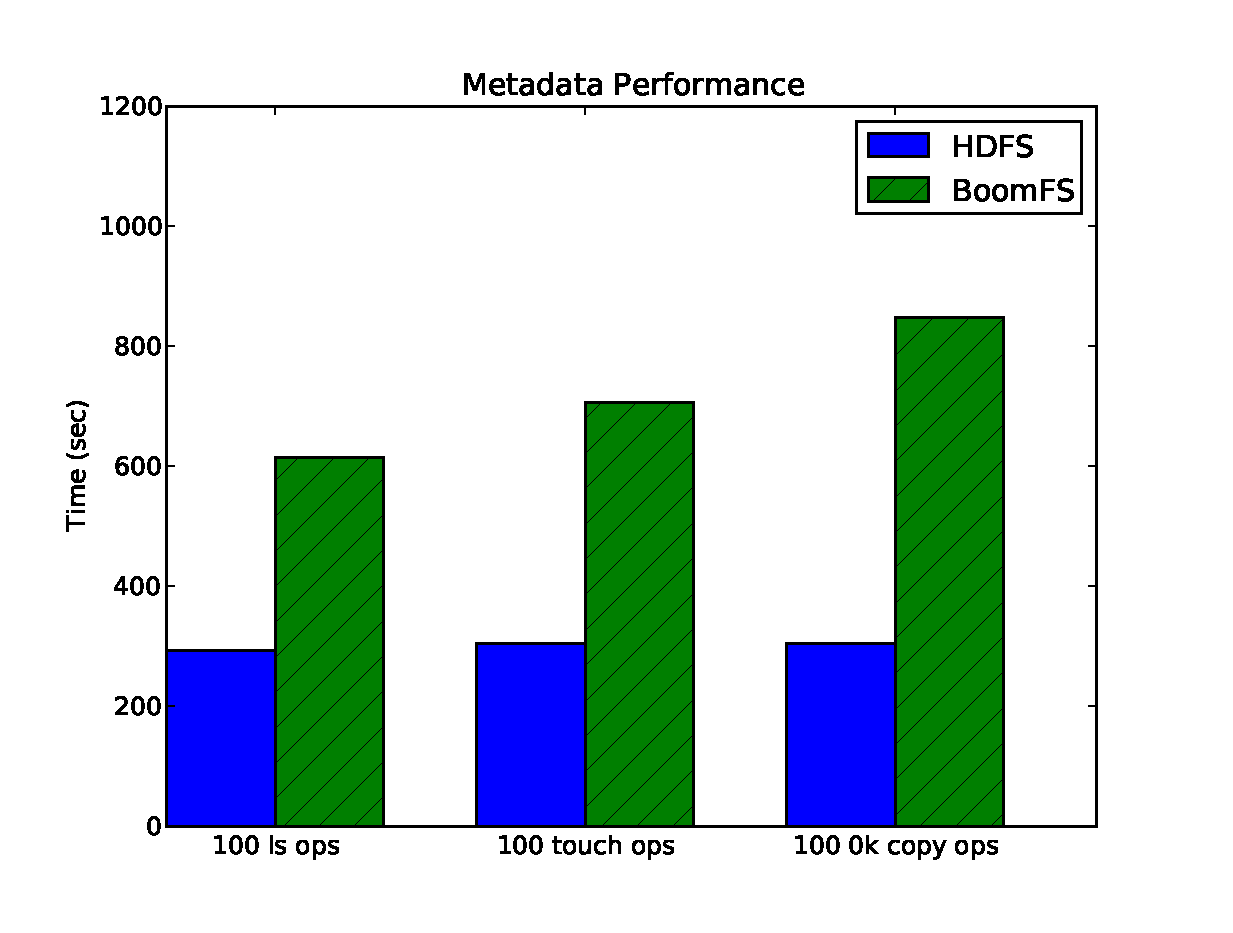
\epsfig{file=figures/metadata_throughput.eps, width=1\columnwidth}
\caption{Performance for metadata operations}
\label{fig:metadata-perf}
\end{figure}

In our first experiment, we compare the latency of metadata operations
affecting the control path.  A directory listing uses the client
protocol and requires a round trip between the client and master and a
lookup on the master, as does touching a file on the filesystem.
Copying a zero-byte file requires two round trips to the master: one
to get a new chunk identifier for the append operation, and another to
request a set of data nodes who can accept the new
chunk.\footnote{Combining these responses into a single message is a
  simple optimization not yet implemented in our prototype.}  The
results of running 100 of each of these metadata operations are shown
in Figure \ref{fig:metadata-perf}.  As we anticipated, the overhead of
these operations is significantly higher in our implementation that in
HDFS.  This is partly due to the current performance of the JOL
implementation. Another factor is the presence of client-side caching,
enabled in HDFS and not yet implemented in BoomFS. However, it would
be simple to locally materialize lookup results into relations that
can be queried before visiting the master.

\subsection{Sort Benchmark}
Our next experiment evaluates read and write performance under a
typical MapReduce workload.  The sort benchmark of Dean and
Ghemawat~\cite{mapreduce} is a simple and practical test that puts
equal stress on the read and write components of a distributed
filesystem.

The MapReduce specification of sorting is trivial, largely because
sorting (over \emph{some} key) is a side-effect of the framework.
Thus, the map function simply returns the sort key and the entire line
as the key's value, and the reduce function is simply the identity
function.  In an execution of the sort, disjoint sections of a single
input file are read in parallel by all of the mappers, which apply the
hash function and write the bucketed results to their local disks.
The reducers then read these files via RPC calls, apply the built-in
merge sort, and write as many files back to the GFS as there are
reducers.

For the purposes of our experiments, we are interested only in the
costs associated with the parallel reads at the start of the workflow
described above, and the parallel writes described at the end.  Hence,
in our simulation we dispense with the actual sorting, hashing and
crossbarring, and focus merely on the filesystem performance as the
number of concurrent clients and data nodes are scaled up together.
For a given concurrency level $D$, we provision an EC2 cluster with a
master node and $D$ data nodes, and prime the filesystem by creating
$D$ 100MB files with a replication factor of 2.  We then spawn $D$
client processes (one on each data node), which read one of the files
from the filesystem, write it to local disk, then create a new
distributed filesystem file and append the contents of the local file
to it.  Thus, each client reads (writes) 100MB to (from) the
filesystem concurrently in each sort benchmark, as we vary $D$.

\begin{figure}
\centering
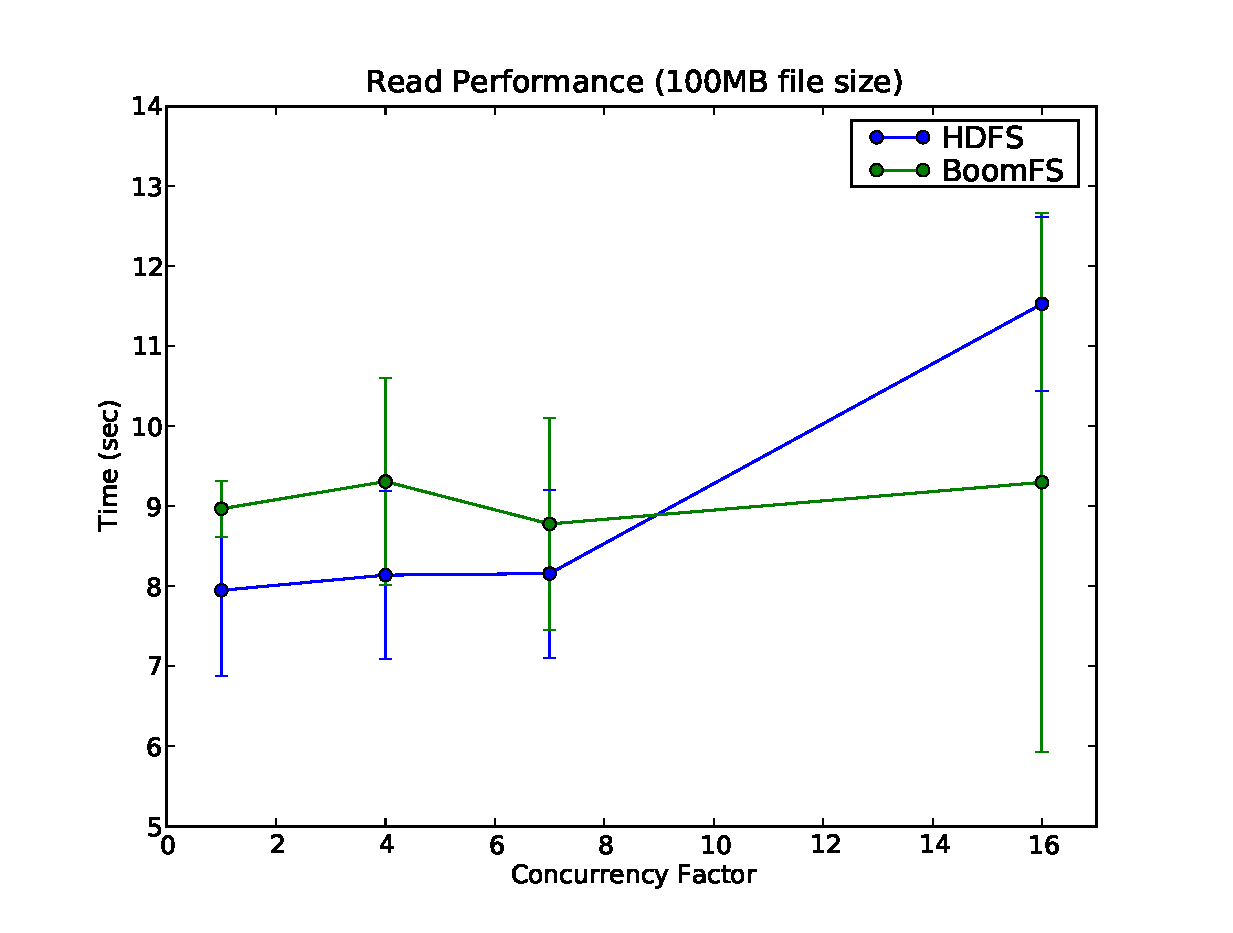
\epsfig{file=figures/big_read_throughput.eps, width=1\columnwidth}
\caption{Sequential read performance for the sort benchmark}
\label{fig:big-read-perf}
\end{figure}
\begin{figure}
\centering
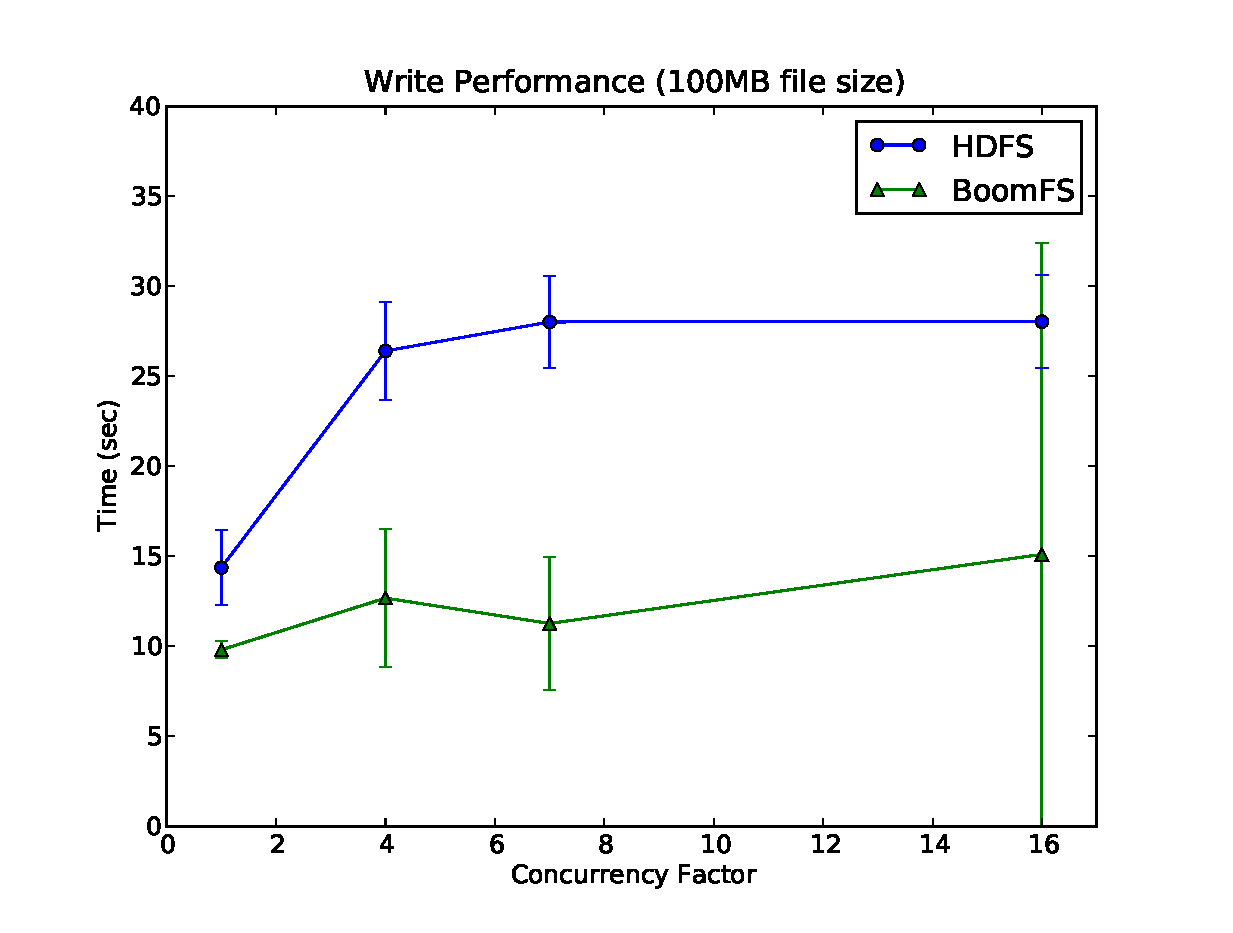
\epsfig{file=figures/big_write_throughput.eps, width=1\columnwidth}
\caption{Sequential write performance for the sort benchmark}
\label{fig:big-write-perf}
\end{figure}
Our results are summarized in Figures \ref{fig:big-read-perf} and
\ref{fig:big-write-perf}.  At lower concurrency levels, BoomFS is
comparable in read performance and handily outperforms HDFS in write
performance.  This result supports our intuition that the relatively
high cost of metadata operations is quickly amortized by the highly
efficient data path under the large transfers characteristic of
MapReduce and Hadoop workloads.

In HDFS, read latency increases gradually as load increases, but write
latency reacts very quickly to concurrency, increasing by almost two
times as we increase the number of clients from 1 to 4.  Beyond that
point, HDFS gracefully handles increasing load, with low variance.
BoomFS shows similar read results, but significantly lower write
latency (less than half that of HDFS, though the variance is higher).

At 16 concurrent clients, the BoomFS implementation began suffering
timeouts.  At this time is is difficult for us to say whether this is
due to issues with queueing in the Overlog runtime implementation,
race conditions or other bugs in the Overlog specification of GFS, or
a problem with the custom data transfer protocol that we implemented.
The variance for $x=16$ in the graph in Figure 4 reflects the fact
that out of 48 observations, 4 timeouts occurred, resulting in write
times greater than 60 seconds (because our timeout was 60 seconds).
If we omit those four observations from our results, the mean write
response time is 10.12 seconds.

\section{Future Work}
\label{future-work}
The current version of the BoomFS prototype confirms that the BOOM
architectural style can be successfully applied to the construction of
a distributed filesystem. However, we feel that the most exciting
research on this topic remains to be done.

We believe that interesting issues in computer system design often
only arise when technology is deployed in production
environments. Therefore, we plan to complete the implementation of
BoomFS and deliver a production-quality filesystem. This requires
implementing support for directories, fine-grained concurrent appends,
and persistent metadata. We also want to ensure that BoomFS is able to
scale to petabyte-range data sets and thousands of nodes. We plan to
validate BoomFS's usability and performance by implementing the HDFS
API, and then using BoomFS to replace HDFS in real-world Hadoop
installations.

We also plan to leverage the flexibility allowed by BoomFS's
declarative specification to explore new filesystem features and
policies. We closely followed the GFS design primarily to demonstrate
that a faithful reimplementation is possible using declarative
techniques, but we plan to consider a much broader space of design
alternatives in the future. For example, it should be possible to
partition the filesystem metadata over the master nodes, removing a
major scalability barrier.

Finally, we plan to explore the cross-layer optimizations that are
enabled when multiple elements of the networking stack are implemented
using the same declarative techniques. For example, colleagues are
completing an implementation of the Hadoop job scheduler in
Overlog. By running this on top of BoomFS, it would be possible for an
optimizer to make intelligent costing decisions for filesystem
operations that automatically reflect the characteristics of the
current Hadoop job.

\section{Related Work}
\label{related-work}
To our knowledge, this work represents the first attempt to specify a
distributed filesystem using declarative techniques. However, it can
be argued that GFS and related designs (including BoomFS) are
``filesystems'' only in a loose sense, because they do not implement
POSIX semantics and provide looser consistency guarantees than
traditional filesystems. In this sense, BoomFS is clearly related to
prior work on declarative specifications of storage infrastructure,
such as DHTs~\cite{chord-overlog} and data replication
systems~\cite{padre-draft}.

Recent work on a declarative filesystem filesystem integrity
checker~\cite{sqck} provides another example of how sophisticated
policies and invariants can be concisely stated in an appropriate
high-level declarative language. Similar tools for distributed
consistency checking, garbage collection, monitoring, and periodic
optimization should be easy to write on top of BoomFS, because all
filesystem metadata is already available for declarative queries. We
plan to explore this topic in the future.

Both BoomFS and GFS emphasize the distinction between control and data
paths. This division has a long history in computer science, and can
be found in protocols ranging from FTP~\cite{ftp-rfc} and
DOT~\cite{dot}, to filesystems like Berkeley FFS~\cite{ffs} and
ext3.\footnote{In these filesystems, metadata and data are subject to
  different consistency requirements and durability guarantees, and
  are implemented using different on-disk data structures.} Similarly,
the separation of control and data is a well-established principle in
computer system design~\cite{hydra-policy-mech-sep}.

\section{Conclusion}
\label{conclusion}
We have implemented BoomFS, a distributed filesystem that is similar
to GFS and HDFS. BoomFS achieves competitive performance with
HDFS. Unlike HDFS, BoomFS avoids a single point of failure through its
support for multiple master nodes and automatic failover.

More importantly, BoomFS is implemented using the BOOM architectural
style: the complex protocols and policy of the control path are
implemented in declarative logic, while the simple, high-performance
data path is written in Java. BoomFS was straightforward to
implement. Because the implementation is concise and comprehensible,
the filesystem is easy to modify and adapt to new environments. BoomFS
is the first of several pieces of data center infrastructure we plan
to implement using declarative techniques as part of the BOOM project.

\bibliographystyle{abbrv}
\bibliography{paper}
\end{document}
